\subsection{Serial}

    \begin{table}[h!]
        \centering
        \small
        \begin{tabular}{|r|r|}
            \hline
            Bo$\backslash$Co & 1 \\\hline
            16   &    0.0250 [s]  \\\hline
            32   &    0.0875 [s]  \\\hline
            64   &    0.3750 [s]  \\\hline
            128  &    1.4625 [s]  \\\hline
            256  &    5.8000 [s]  \\\hline
            512  &   23.4750 [s]  \\\hline
            1024 &   93.7375 [s]  \\\hline
            2048 &  374.6500 [s]  \\\hline
            4096 & 1478.3620 [s]  \\\hline
        \end{tabular}
        \caption{Serial best test results}
        \label{tab:serial}
    \end{table}

\subsection{OpenMP}

    \begin{table}[h!]
        \centering
        \small
        \begin{tabular}{|l|r|r|r|r|r|r|r|r|r|}
            \hline
            Bo$\backslash$Co & 1             & 2             & 4             & 6            & 8             \\\hline
            16               & \blue{0.0125} [s]    & 0.0250 [s]    & 0.0250 [s]    & 0.0375 [s]   & 0.0500 [s]    \\\hline
            32               & 0.0875 [s]    & 0.1125 [s]    & 0.1125 [s]    & 0.0876 [s]   & \blue{0.0625} [s]    \\\hline
            64               & 0.4750 [s]    & 0.5125 [s]    & 0.3375 [s]    & 0.3000 [s]   & 0.275  [s]    \\\hline
            128              & 1.7375 [s]    & 2.0375 [s]    & 1.3375 [s]    & 1.2125 [s]   & 1.0500 [s]    \\\hline
            256              & 7.2250 [s]    & 7.7375 [s]    & 5.4500 [s]    & 4.7875 [s]   & 4.1875 [s]    \\\hline
            512              & 27.4375 [s]   & 31.9750 [s]   & 21.4875 [s]   & 18.5250 [s]  & 16.5000 [s]   \\\hline
            1024             & 102.5626 [s]  & 126.4626 [s]  & 84.1250 [s]   & 72.2625 [s]  & 65.9000 [s]   \\\hline
            2048             & 428.2626 [s]  & 503.8750 [s]  & 335.2248 [s]  & 293.4126 [s] & 263.1998 [s]  \\\hline
            4096             & 1605.1980 [s] & 2000.6500 [s] & 1326.6500 [s] & 1149.6480[s] & 1044.0740 [s] \\\hline
        \end{tabular}
        \caption{OpenMP best test results (1/2)}
        \label{tab:openmp}
    \end{table}

    \begin{table}[h!]
        \centering
        \small
        \begin{tabular}{|l|r|r|r|r|r|r|r|r|r|}
            \hline
            Bo$\backslash$Co & 10           & 12           & 14           & 16           \\\hline
            16               & 0.0620 [s]   & 0.0625 [s]   & 0.0625 [s]   & 0.0625 [s]   \\\hline
            32               & 0.0750 [s]   & 0.0750 [s]   & 0.0625 [s]   & 0.0875 [s]   \\\hline
            64               & 0.2375 [s]   & 0.2125 [s]   & 0.2000 [s]   & \blue{0.1875} [s]   \\\hline
            128              & 0.9000 [s]   & 0.7750 [s]   & 0.7375 [s]   & \blue{0.6625} [s]   \\\hline
            256              & 3.5375 [s]   & 3.0625 [s]   & 2.5750 [s]   & \blue{2.3125} [s]   \\\hline
            512              & 13.9875 [s]  & 11.7625  [s] & 10.1750 [s]  & \blue{8.9125} [s]   \\\hline
            1024             & 54.5625 [s]  & 46.6250  [s] & 40.5375 [s]  & \blue{35.6125} [s]  \\\hline
            2048             & 221.0252 [s] & 184.1752 [s] & 160.7498 [s] & \blue{143.0376} [s] \\\hline
            4096             & 871.7500 [s] & 737.2500 [s] & 638.3750 [s] & \blue{568.0000} [s] \\\hline
        \end{tabular}
        \caption{OpenMP best test results (2/2)}
        \label{tab:openmp}
    \end{table}

\newpage
\subsection{POSIX Threads}


    \begin{table}[h!]
        \centering
        \small
        \begin{tabular}{|l|r|r|r|r|r|r|r|r|r|}
            \hline
            Bo $\backslash$Co & 1             & 2            & 4            & 6            & 8             \\\hline
            16                & 0.0625 [s]    & 0.0625 [s]   & 0.0625 [s]   & \blue{0.0125} [s]   & 0.1625 [s]    \\\hline
            32                & \blue{0.1250} [s]    & 0.1250 [s]   & 0.1500 [s]   & 0.1875 [s]   & 0.2125 [s]    \\\hline
            64                & 0.4750 [s]    & \blue{0.2625} [s]   & 0.3750 [s]   & 0.3875 [s]   & 0.4250 [s]    \\\hline
            128               & 1.5250 [s]    & \blue{1.0125} [s]   & 1.0250 [s]   & 1.0375 [s]   & 1.0500 [s]    \\\hline
            256               & 5.6250 [s]    & 3.3750 [s]   & 2.4000 [s]   & \blue{2.2375} [s]   & 2.5625 [s]    \\\hline
            512               & 22.0125 [s]   & 11.9875 [s]  & 7.0750 [s]   & 5.6250 [s]   & 5.4000 [s]    \\\hline
            1024              & 85.9500 [s]   & 47.0875 [s]  & 24.4250 [s]  & 18.2250 [s]  & 15.4375 [s]   \\\hline
            2048              & 335.0500 [s]  & 188.0876 [s] & 93.7375 [s]  & 65.1125 [s]  & 53.2125 [s]   \\\hline
            4096              & 1364.0000 [s] & 750.2500 [s] & 353.3750 [s] & 243.7500 [s] & 178.8750 [s]  \\\hline
        \end{tabular}
        \caption{Pthreads best test results (1/2)}
        \label{tab:pthreads}
    \end{table}

    \begin{table}[h!]
        \centering
        \small
        \begin{tabular}{|l|r|r|r|r|r|r|r|r|r|}
            \hline
            Bo $\backslash$Co & 10           & 12           & 14           & 16 \\\hline
            16                & 0.2250 [s]   & 0.2750 [s]   & 0.3125 [s]   & 0.3750 [s] \\\hline
            32                & 0.2625 [s]   & 0.3000 [s]   & 0.3750 [s]   & 0.4000 [s] \\\hline
            64                & 0.4375 [s]   & 0.5000 [s]   & 0.5000 [s]   & 0.5875 [s] \\\hline
            128               & 1.0625 [s]   & 1.0875 [s]   & 1.1625 [s]   & 1.2250 [s] \\\hline
            256               & 2.5250 [s]   & 2.6000 [s]   & 2.5500 [s]   & 2.8250 [s] \\\hline
            512               & 5.5375 [s]   & 5.4875 [s]   & \blue{5.3250} [s]   & 5.5500 [s] \\\hline
            1024              & 14.3000 [s]  & 14.1750 [s]  & 14.0250 [s]  & \blue{14.0000} [s] \\\hline
            2048              & 46.4500 [s]  & 41.3375 [s]  & \blue{39.2250} [s]  & 42.1750 [s] \\\hline
            4096              & 172.3750 [s] & 147.3750 [s] & 134.6250 [s] & \blue{129.1250} [s] \\\hline
        \end{tabular}
        \caption{Pthreads best test results (2/2)}
        \label{tab:pthreads}
    \end{table}

\subsection{CUDA}

    \begin{table}[h!]
        \centering
        \small
        \begin{tabular}{|r|r|r|r|}
            \hline
            Bo$\backslash$ CUDA config & & BpG & TpB \\ \hline
            16    &   0.0494   &   1  &  32 \\\hline
            32    &   0.1024   &   1  &  32 \\\hline
            64    &   0.1976   &   2  &  32 \\\hline
            128   &   0.3871   &   4  &  32 \\\hline
            256   &   0.8017   &   8  &  32 \\\hline
            512   &   1.9284   &  16  &  32 \\\hline
            1024  &   5.6289   &  32  &  32 \\\hline
            2048  &  20.9967   &  64  &  32 \\\hline
            4096  &  82.1908   & 128  &  32 \\\hline
        \end{tabular}
        \caption{CUDA best test results}
        \label{tab:cuda}
    \end{table}

\subsection{CUDA and PThreads}

The following plots \ref{fig:pthvscuda1} and \ref{fig:pthvscuda2} show a comparison between the Pthreads and CUDA implementation.
This approaches implementation are based in two different algoritgm type,
fine and coarse grained.

The implementations looking for an scenario in which each technology
is benefited; coarse grain for the CPU and fine grain for the GPU.

\begin{figure}
    \centering
    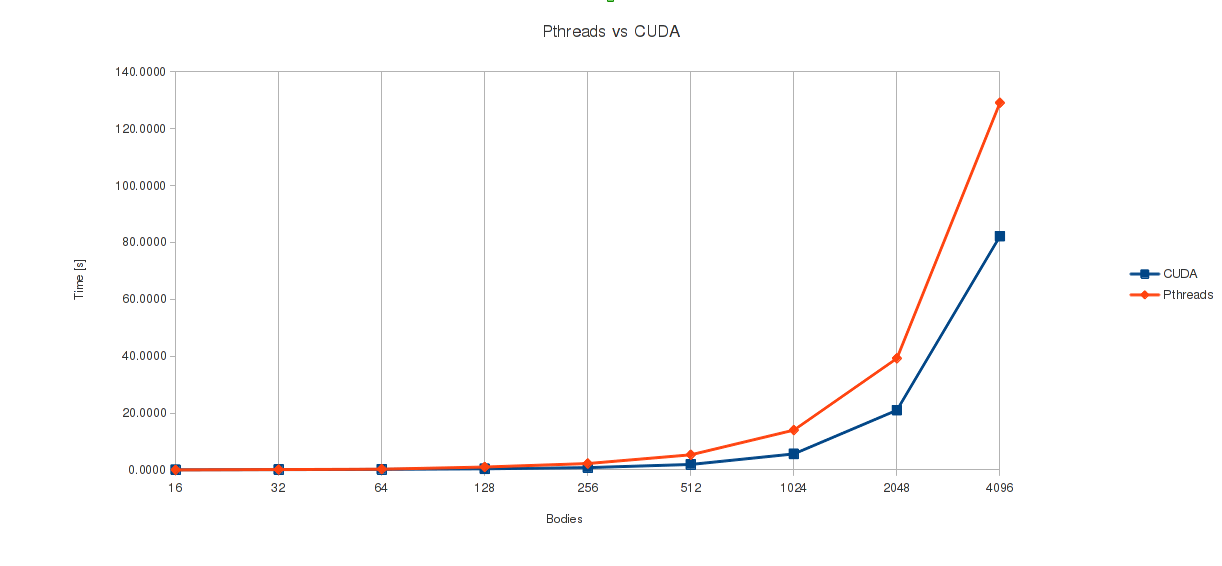
\includegraphics[width=0.9\textwidth]{img/pthvscuda-4096}
    \caption{Pthreads vs CUDA until 4096 bodies}
    \label{fig:pthvscuda1}
\end{figure}

\begin{figure}
    \centering
    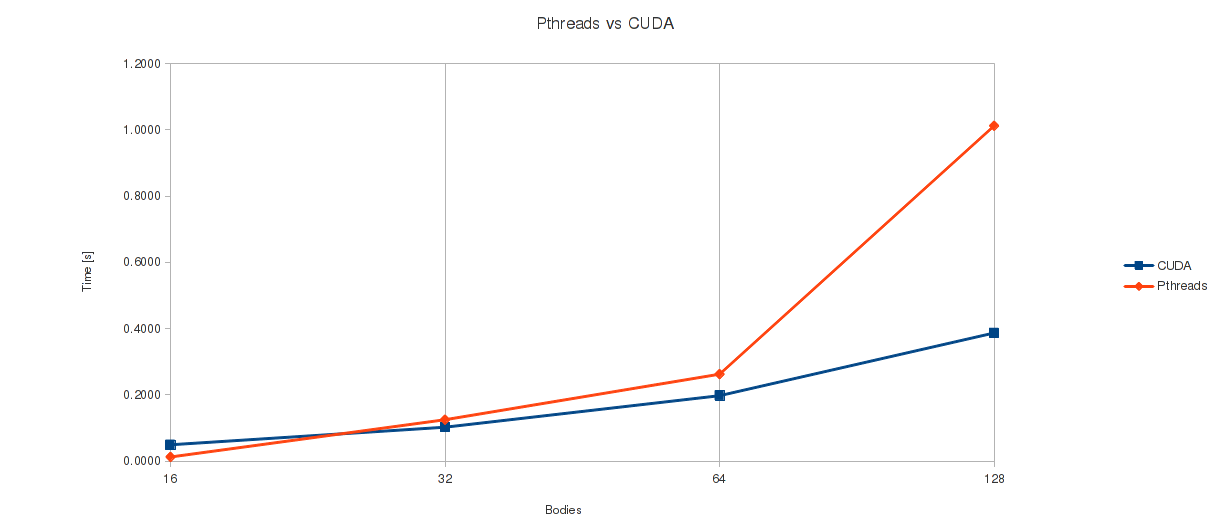
\includegraphics[width=0.9\textwidth]{img/pthvscuda-128}
    \caption{Pthreads vs CUDA until 128 bodies}
    \label{fig:pthvscuda2}
\end{figure}
